\documentclass[floatsintext,man]{apa6}

\usepackage{amssymb,amsmath}
\usepackage{ifxetex,ifluatex}
\usepackage{fixltx2e} % provides \textsubscript
\ifnum 0\ifxetex 1\fi\ifluatex 1\fi=0 % if pdftex
  \usepackage[T1]{fontenc}
  \usepackage[utf8]{inputenc}
\else % if luatex or xelatex
  \ifxetex
    \usepackage{mathspec}
    \usepackage{xltxtra,xunicode}
  \else
    \usepackage{fontspec}
  \fi
  \defaultfontfeatures{Mapping=tex-text,Scale=MatchLowercase}
  \newcommand{\euro}{€}
\fi
% use upquote if available, for straight quotes in verbatim environments
\IfFileExists{upquote.sty}{\usepackage{upquote}}{}
% use microtype if available
\IfFileExists{microtype.sty}{\usepackage{microtype}}{}

% Table formatting
\usepackage{longtable, booktabs}
\usepackage{lscape}
% \usepackage[counterclockwise]{rotating}   % Landscape page setup for large tables
\usepackage{multirow}		% Table styling
\usepackage{tabularx}		% Control Column width
\usepackage[flushleft]{threeparttable}	% Allows for three part tables with a specified notes section
\usepackage{threeparttablex}            % Lets threeparttable work with longtable

% Create new environments so endfloat can handle them
% \newenvironment{ltable}
%   {\begin{landscape}\begin{center}\begin{threeparttable}}
%   {\end{threeparttable}\end{center}\end{landscape}}

\newenvironment{lltable}
  {\begin{landscape}\begin{center}\begin{ThreePartTable}}
  {\end{ThreePartTable}\end{center}\end{landscape}}




% The following enables adjusting longtable caption width to table width
% Solution found at http://golatex.de/longtable-mit-caption-so-breit-wie-die-tabelle-t15767.html
\makeatletter
\newcommand\LastLTentrywidth{1em}
\newlength\longtablewidth
\setlength{\longtablewidth}{1in}
\newcommand\getlongtablewidth{%
 \begingroup
  \ifcsname LT@\roman{LT@tables}\endcsname
  \global\longtablewidth=0pt
  \renewcommand\LT@entry[2]{\global\advance\longtablewidth by ##2\relax\gdef\LastLTentrywidth{##2}}%
  \@nameuse{LT@\roman{LT@tables}}%
  \fi
\endgroup}


  \usepackage{graphicx}
  \makeatletter
  \def\maxwidth{\ifdim\Gin@nat@width>\linewidth\linewidth\else\Gin@nat@width\fi}
  \def\maxheight{\ifdim\Gin@nat@height>\textheight\textheight\else\Gin@nat@height\fi}
  \makeatother
  % Scale images if necessary, so that they will not overflow the page
  % margins by default, and it is still possible to overwrite the defaults
  % using explicit options in \includegraphics[width, height, ...]{}
  \setkeys{Gin}{width=\maxwidth,height=\maxheight,keepaspectratio}
\ifxetex
  \usepackage[setpagesize=false, % page size defined by xetex
              unicode=false, % unicode breaks when used with xetex
              xetex]{hyperref}
\else
  \usepackage[unicode=true]{hyperref}
\fi
\hypersetup{breaklinks=true,
            pdfauthor={},
            pdftitle={The effect of linking assumptions and number of response options on inferred scalar implicature rate},
            colorlinks=true,
            citecolor=blue,
            urlcolor=blue,
            linkcolor=black,
            pdfborder={0 0 0}}
\urlstyle{same}  % don't use monospace font for urls

\setlength{\parindent}{0pt}
%\setlength{\parskip}{0pt plus 0pt minus 0pt}

\setlength{\emergencystretch}{3em}  % prevent overfull lines


% Manuscript styling
\captionsetup{font=singlespacing,justification=justified}
\usepackage{csquotes}
\usepackage{upgreek}

 % Line numbering
  \usepackage{lineno}
  \linenumbers


\usepackage{tikz} % Variable definition to generate author note

% fix for \tightlist problem in pandoc 1.14
\providecommand{\tightlist}{%
  \setlength{\itemsep}{0pt}\setlength{\parskip}{0pt}}

% Essential manuscript parts
  \title{The effect of linking assumptions and number of response options on
inferred scalar implicature rate}

  \shorttitle{Linking assumptions and implicature rate}


  \author{Masoud Jasbi\textsuperscript{1}, Brandon Waldon\textsuperscript{1}, \& Judith Degen\textsuperscript{1}}

  % \def\affdep{{"", "", ""}}%
  % \def\affcity{{"", "", ""}}%

  \affiliation{
    \vspace{0.5cm}
          \textsuperscript{1} Stanford University  }

  \authornote{
    Add complete departmental affiliations for each author here. Each new
    line herein must be indented, like this line. Enter author note here.
    
    Correspondence concerning this article should be addressed to Masoud
    Jasbi, Postal address. E-mail:
    \href{mailto:my@email.com}{\nolinkurl{my@email.com}}
  }


  \abstract{Enter abstract here. Each new line herein must be indented, like this
line.}
  \keywords{scalar implicature; methodology; linking assumption; experimental
pragmatics; truth-value judgment task \\

    \indent Word count: X
  }





\usepackage{amsthm}
\newtheorem{theorem}{Theorem}
\newtheorem{lemma}{Lemma}
\theoremstyle{definition}
\newtheorem{definition}{Definition}
\newtheorem{corollary}{Corollary}
\newtheorem{proposition}{Proposition}
\theoremstyle{definition}
\newtheorem{example}{Example}
\theoremstyle{definition}
\newtheorem{exercise}{Exercise}
\theoremstyle{remark}
\newtheorem*{remark}{Remark}
\newtheorem*{solution}{Solution}
\begin{document}

\maketitle

\setcounter{secnumdepth}{0}



\section{Introduction}\label{introduction}

The past 15 years have seen the rise and development of a bustling and
exciting new field at the intersection of linguistics, psychology, and
philosophy: \emph{experimental pragmatics} (Bott \& Noveck, 2004;
Breheny, Katsos, \& Williams, 2006; Degen \& Tanenhaus, 2015; Geurts \&
Pouscoulous, 2009; Grodner, Klein, Carbary, \& Tanenhaus, 2010; Huang \&
Snedeker, 2009; I. A. Noveck \& Reboul, 2008) \textbf{XXX ADD MORE}.
Experimental pragmatics is devoted to experimentally testing theories of
how language is used in context. How do listeners draw inferences about
the -- often underspecified -- linguistic signal they receive from
speakers? How do speakers choose between the many utterance alternatives
they have at their disposal?

The most prominently studied phenomenon in experimental pragmatics is
undoubtedly \emph{scalar implicature}. Scalar implicatures arise in
virtue of a speaker producing the weaker of two ordered scalemates
(hornXXX; {\textbf{???}}, {\textbf{???}}; Grice, 1975). Examples are
provided in (1) and (2).

\begin{enumerate}
\def\labelenumi{\arabic{enumi}.}
\item
\end{enumerate}

\begin{itemize}
\tightlist
\item
  \emph{Utterance:} Some of her pets are cats.
\item
  \emph{Implicature:} Some, but not all, of her pets are cats.
\item
  \emph{Scale:} 
\end{itemize}

\begin{enumerate}
\def\labelenumi{\arabic{enumi}.}
\setcounter{enumi}{1}
\item
\end{enumerate}

\begin{itemize}
\tightlist
\item
  \emph{Utterance:} She owns a cat or a dog.
\item
  \emph{Implicature:} She owns a cat or a dog, but not both.
\item
  \emph{Scale:} 
\end{itemize}

A listener, upon observing the utterances in (1a) and (2a), typically
infers that the speaker intended to convey the meanings in (1b) and
(2b), respectively. Since Grice (1975), the agreed-upon abstract
rationalization the listener could give for their inference goes
something like this: the speaker could have made a more informative
statement by producing the stronger alternative (e.g., \emph{All of her
pets are cats.}). If the stronger alternative is true, they should have
produced it to comply with the Cooperative Principle. They chose not to.
I believe the speaker knows whether the stronger alternative is true.
Hence, it must not be true.

Because the basic reconstruction of the inference is much more easily
characterized for scalar implicatures than for other implicatures,
scalar implicatures have served as a test bed for many questions in
experimental pragmatics, including, but not limited to:

\begin{enumerate}
\def\labelenumi{\arabic{enumi}.}
\item
  Are scalar inferences default inferences, in the sense that they arise
  unless blocked by (marked) contexts (Degen, 2015; Horn, 1984;
  Levinson, 2000)?
\item
  Are scalar inferences default inferences, in the sense that they are
  computed automatically in online processing and only cancelled by
  context in a second effortful step if required by context) {[}Bott and
  Noveck (2004);Breheny et al. (2006);Degen and Tanenhaus (2016);Grodner
  et al. (2010);Huang and Snedeker (2009);Politzer-Ahles and Fiorentino
  (2013);Tomlinson2013{]}?
\item
  What are the (linguistic and extra-linguistic) factors that affect
  whether a scalar implicature is derived {[}Zondervan (2010);Degen and
  Tanenhaus (2015); Degen and Tanenhaus (2016); Degen (2015); Degen and
  Goodman (2014); Bergen and Grodner (2012); Breheny et al. (2006);
  Breheny, Ferguson, and Katsos (2013);Marneffe and Tonhauser (2016);De
  Neys and Schaeken (2007);Bonnefon, Feeney, and Villejoubert
  (2009);Chemla2011;Potts2015{]}?
\item
  How much diversity is there across implicature types, and within
  scalar implicatures across scale types, in whether or not an
  implicature is computed (Doran, Ward, Larson, McNabb, \& Baker, 2012;
  Tiel, Miltenburg, Zevakhina, \& Geurts, 2014)?
\item
  At what age do children acquire the ability to compute implicatures
  (Barner, Brooks, \& Bale, 2011; Katsos \& Bishop, 2011; Frank;
  Musolino, 2004; Noveck, 2001; Papafragou \& Tantalou, 2004)?
\end{enumerate}

In addressing all of these questions, it has been crucial to obtain
estimates of \textbf{implicature rates}. For 1., implicature rates from
experimental tasks can be taken to inform whether scalar implicatures
should be considered default inferences. For 2., processing measures on
responses that indicate implicatures can be compared to processing
measures on responses that indicate literal interpretations. For 3.,
contextual effects can be examined by comparing implicature rates across
contexts. For 4., implicature rates can be compared across scales (or
across implicature types). For 5., implicature rates can be compared
across age groups.

A standard measure that has stood proxy for implicature rate across many
studies is the proportion of \enquote{pragmatic} judgments in
truth-value judgment paradigms {[}Bott and Noveck (2004);Noveck
(2001);Noveck and Posada (2003);Chemla and Spector (2011);Geurts and
Pouscoulous (2009);Degen and Tanenhaus (2015);De Neys and Schaeken
(2007);Degen2014{]}. In these kinds of tasks, participants are provided
a set of facts, either presented visually or via their own knowledge of
the world. They are then asked to judge whether a sentence intended to
describe those facts is true or false (or alternatively, whether it is
right or wrong, or they are asked whether they agree or disagree with
the sentence). The crucial condition for assessing implicature rates in
these kinds of studies typically consists of a case where the facts are
such that the stronger alternative is true and the target utterance is
thus also true but underinformative. For instance, Bott and Noveck
(2004) asked participants to judge sentences like \enquote{Some
elephants are mammals}, when world knowledge dictates that all elephants
are mammals. Similarly, Degen and Tanenhaus (2015) asked participants to
judge sentences like \enquote{You got some of the gumballs} in
situations where the visual evidence indicated that the participant
received all the gumballs from a gumball machine. In these kinds of
scenarios, the story goes, if a participant responds \enquote{FALSE},
that indicates that they computed a scalar implicature, eg to the effect
of \enquote{Not all elephants are mammals} or \enquote{You didn't get
all of the gumballs}, which is (globally or contextually) false. If
instead a participant responds \enquote{TRUE}, that is taken to indicate
that they interpreted the utterance literally as `Some, and possibly
all, elephants are mammals' or \enquote{You got some, and possibly all,
of the gumballs}.

Given the centrality of the theoretical notion of \enquote{implicature
rate} to much of experimental pragmatics, there is to date a surprising
lack of discussion of the basic assumption that it is adequately
captured by the proportion of FALSE responses in truth-value judgment
tasks (but see ({\textbf{???}}); Geurts and Pouscoulous (2009); Degen
and Goodman (2014); Katsos and Bishop (2011)). Indeed, the scalar
implicature acquisition literature was shaken up when Katsos and Bishop
(2011) showed that simply by introducing an additional response option,
children started looking much more pragmatic than had been previously
observed in a binary judgment paradigm. ({\textbf{???}}) allowed
children to distribute 1, 2, or 3 strawberries to a puppet depending on
\enquote{how good the puppet said it}. The result was that children gave
on average fewer strawberries to the puppet when he produced
underinformative utterances compared to when he produced literally true
and pragmatically felicitous utterances, suggesting that children do, in
fact, display pragmatic ability even at ages when they had previously
appeared not to.

But this raises an important question: in truth-value judgment task, how
do we know whether an interpretation is literal or the result of an
implicature computation? The binary choice task typically used is
appealing in part because it allows for a direct mapping from response
options -- TRUE and FALSE -- to interpretations -- literal and
pragmatic. That the seeming simplicity of this mapping is illusory
becomes apparent once a third response option is introduced, as in the
Katsos and Bishop (2011) case. How is the researcher to interpret the
intermediate option? Katsos and Bishop (2011) grouped the intermediate
option with the negative endpoint of the scale for the purpose of
categorizing judgments as literal vs.~pragmatic. But it seems just as
plausible that they could have grouped it with the positive endpoint of
the scale and taken the hard line that only truly FALSE responses
constitute a full-fledged implicature. The point here is that there has
been remarkably little consideration of \textbf{linking functions}
between behavioral measures and theoretical constructs in experimental
pragmatics, a problem in many subfields of psycholinguistics
({\textbf{???}}). We argue that it is time to engage more seriously with
these issues.

We begin by reporting an experiment that addresses the following
question: do the number of response options provided in a truth-value
judgment task and the way that responses are grouped into pragmatic
(\enquote{SI}) and literal (\enquote{no SI}) change inferences about
scalar implicature rates? Note that this way of asking the question
presupposes two things: first, that whatever participants are doing in a
truth-value judgment task, the behavioral measure can be interpreted as
providing a measure of \textbf{interpretation}. And second, that
listeners either do or do not compute an implicature on any given
occasion. In the Discussion we will discuss both of these issues. First,
following Degen and Goodman (2014), we will offer some remarks on why
truth-value judgment tasks are better thought of as measuring
participants' estimates of speakers' \textbf{production} probabilities.
This will suggest a completely different class of linking functions. And
second, we discuss an alternative conception of scalar implicature as a
probabilistic phenomeonen, a view that has recently rose to prominence
in the subfield of probabilistic pragmatics. This alternative conception
of scalar implicature, we argue, affords developing and testing
quantitative linking functions in a rigorous and motivated way.

Consider a setup in which a listener is presented a card with a
depiction of either one or two animals (see the figure below for an
example). As in a standard truth-value judgment task, the listener then
observes an underinformative utterance about this card (e.g.,
\enquote{There is a cat or a dog on the card}) and is asked to provide a
judgment on a scale from 2 to 5 response options, with endpoints
\enquote{wrong} and \enquote{right}. In the binary case, this reproduces
the standard truth-value judgment task. \textbf{XXX say briefly sth
about wrong/right vs true/false and agree/disagree}. The figure below
exemplifies (some of) the researcher's options for grouping responses.
Under what we will call the \enquote{Strong link} assumption, only the
negative endpoint of the scale is interpreted as evidence for a scalar
implicature having been computed. Under the \enquote{Weak link}
assumption, in contrast, any response that does not correspond to the
positive endpoint of the scale is interpreted as evidence for a scalar
implicature having been computed. Intermediate grouping schemes are also
possible, but these are the ones we will consider here. Note that for
the binary case, the Weak and Strong link return the same categorization
scheme, but for any number of response options greater than 2, the Weak
and Strong link can in principle lead to differences in inferences about
implicature rate.

\begin{figure}
\centering
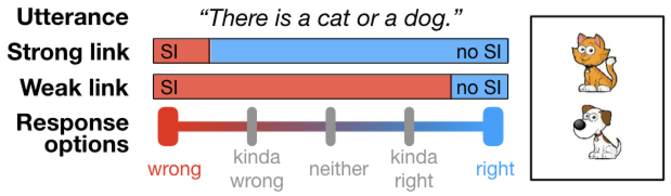
\includegraphics{writeup_files/figure-latex/linkvisualization-1.pdf}
\caption{\label{fig:linkvisualization}Strong and weak link from response
options to researcher inference about scalar implicature rate,
exemplified for the disjunctive utterance when the conjunction is true.}
\end{figure}

Let's examine an example. Assume three response options (wrong, neither,
right). Assume further that a third of participants each gave each of
the three responses, i.e., the distributions of responses is 1/3, 1/3,
and 1/3. Under the Strong link, we infer that this task yielded an
implicature rate of 2/3. Under the Weak link, we infer that this task
yielded an implicature rate of 1/3. This is quite a drastic difference
if we are for instance interested in whether scalar implicatures are
inference defaults and we would like to interpret an implicature rate of
above an arbitrary threshold (e.g., 50\%) as evidence for such a claim.
Under the Strong link, we would conclude that scalar implicatures are
not defaults. Under the Weak link, we would conclude that they are.

In the experiment reported in the following section, we presented
participants with exactly this setup. Different groups of participants
were presented with different numbers of response options. We
categorized their responses according to the Weak and the Strong link
and tested whether number of response options and categorization scheme
leads to different conclusions about implicature rates.

\section{Experiment}\label{experiment}

\subsection{Methods}\label{methods}

\subsubsection{Participants}\label{participants}

200 participants were recruited using Amazon Mechanical Turk (binary=50,
ternary53, quaternary=43, quinary=54). No participant was excluded from
the final analysis.

\subsubsection{Procedure}\label{procedure}

The study was administered online through Amazon Mechanical Turk.
Participants were introduced to a set of cards with pictures of one or
two animals (Figure \ref{fig:stimuli}). They were told that a
blindfolded fictional character called Bob is going to guess what
animals are on the card. On each trial, participants saw a card as well
as a sentence representing Bob's guess. For example, they saw a card
with a cat on it and read the sentence \enquote{There is a cat on the
card.} The study ended after 24 trials. At the end participants
optionally provided demographic information. We also asked participants
if they had any prior training in logic. You can access and view on the
study's \href{https://github.com/thegricean/si-paradigms/}{online
repository}.

\subsubsection{Design and Materials}\label{design-and-materials}

\begin{figure}
\centering
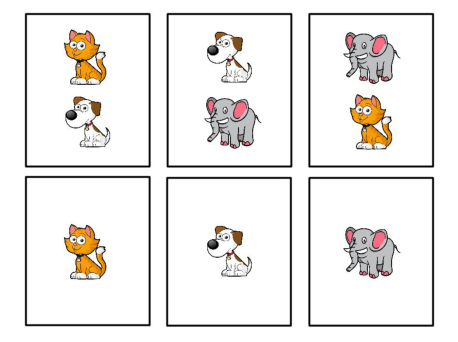
\includegraphics{writeup_files/figure-latex/stimuli-1.pdf}
\caption{\label{fig:stimuli}Cards used in the connective guessing game.}
\end{figure}

The study had two main manipulaitons within participants: the type of
card and the type of guess. There were two types of cards. Cards with
only one animal on them and cards with two animals. Animals were chosen
from the following set: cat, dog, and elephant There were three types of
guesses: simple (e.g. \emph{There is a cat}), conjunctive (e.g.
\emph{There is a cat and a dog}), and disjunctive (e.g. \emph{There is a
cat or a dog}). In each trial, the animal labels used in the guess and
the animal images on the card may have no overlap (e.g.~Image: cat,
Guess: \emph{There is an elephant}), a partial overlap (e.g.~Image: cat,
Guess: \emph{There is a cat or a dog}), or a total overlap (e.g.~Image:
cat and dog, Guess: \emph{There is a cat or a dog}). Crossing the number
of animals on the card, the type of guess, and the overlap between the
guess and the card results in 12 different possible trial types. We
chose 8 trial types (Figure \ref{fig:trials}), balancing the number of
one-animal vs.~two-animal cards, simple vs.~connective guesses, and
expected true vs.~false trials. Three trials were randomly selected from
each of the 8 trial-types, for a total of 24 trials. The order of these
24 trials was randomized as well.

Participants could derive implicatures in two trial types. First, the
trial type in which two animals were present on the card (e.g.~cat and
dog) but Bob guessed only one of them (e.g. \enquote{there is a cat}).
Such trials can have a literal interpretation (cat and possibly more) or
an exhaustive interpretation (only cat). We refer to them as
\enquote{exhaustive}. The second trial type with implicatures was the
one in which two animals were on the card (e.g.~cat and dog) and Bob
used a disjunciton (e.g.~cat or dog). These trials can have a literal
(inclusive) interpretation (e.g.~cat or dog or both), or an exclusive
interpretation (e.g.~cat or dog, not both). We refer to these trials as
\enquote{scalar}. The following four trial types were used as
experimental control: two trial types where there was no overlap between
the guess (e.g.~elephant) and the animal(s) on the card (e.g.~cat, cat
and dog); and two trial types where the animal(s) on the card were
correctly guessed. For example, if there was only a cat on the card, Bob
said \enquote{there is a cat} and if there was a cat and a dog, Bob said
\enquote{there is a cat and a dog}. Since the fictional character was
blindfolded and did not see the outcome of the game, the ignorance
inference commonly associated with disjunction was already common ground
in the experimental setting. If the character was seeing the cards or
knew what was on them, a disjunction would have violated the expectation
that the speaker does not know which alternative actually holds. Our
study controls for the possibile effect of ignorance violations on
exclusivity and exhaustive inferences.

The study also had a between participant manipulation of the number of
response options in the forced choice task. Participants were randomly
assigned to one of four different conditions. The conditions differed
with respect to the number of response options: binary (wrong
vs.~right), ternary (wrong, neither, right), quaternary (wrong, kinda
wrong, kinda right, right), and quinary (wrong, kinda wrong, neither,
kinda right, right). We wanted to see if the number of response options
in the forced choice task would affect our estimate of the task's
\enquote{implicature rate}.

\begin{figure}
\centering
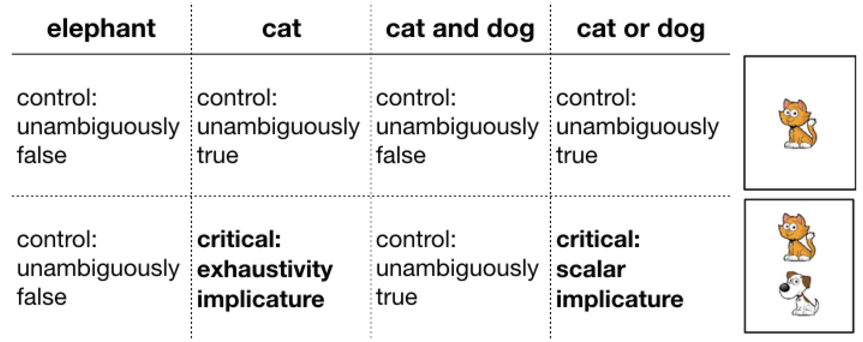
\includegraphics{writeup_files/figure-latex/trials-1.pdf}
\caption{\label{fig:trials}Trial types represented by example cards and
guesses.}
\end{figure}

\subsection{Results}\label{results}

\begin{figure}
\centering
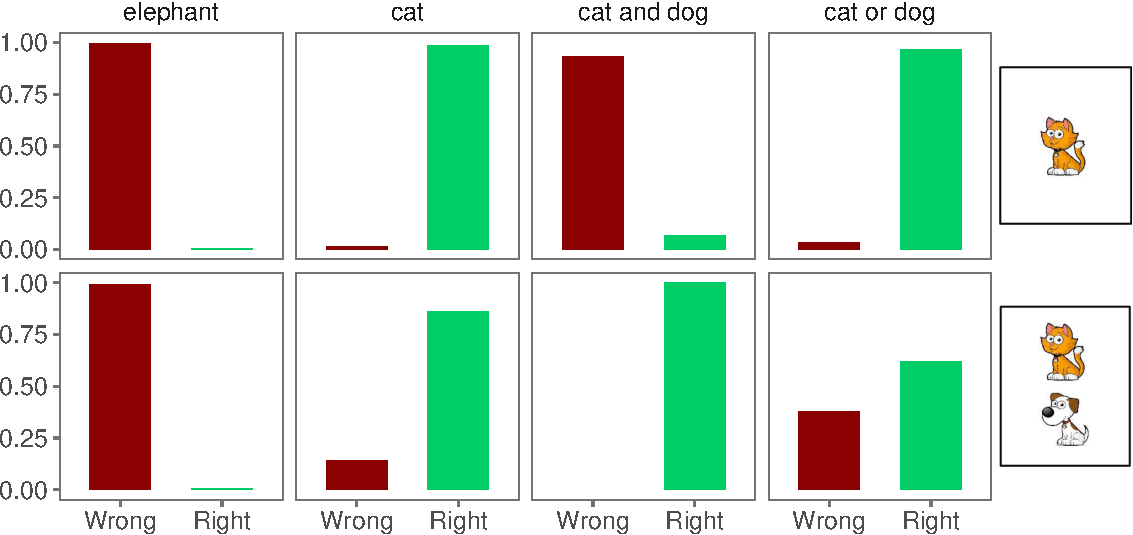
\includegraphics{writeup_files/figure-latex/binaryPlot-1.pdf}
\caption{\label{fig:binaryPlot}Proportion responses for the two-alternative
(binary) forced choice judgments in the guessing game.}
\end{figure}

Here we present the proportion that participants chose the response
options in each of the 8 trial types of the binary, ternary, quaternary,
and quinary tasks. Figure \ref{fig:binaryPlot} shows the proportion of
\enquote{right} and \enquote{wrong} responses in the binary task.
Starting from the leftmost column, participants considered a guess
\enquote{wrong} if the guessed animal was not on the card. Moving to the
second column, participants considered a guess \enquote{right} if the
animal on the card was mentioned. However, if only one of the two
animals on the card was mentioned (exhaustive trials), 14\% of the times
participants considered the guess \enquote{wrong}. Moving to the third
column, if a conjunction of animals was guessed while only one animal
was on the card, participants considered the guess to be
\enquote{wrong}. If a conjunction of animals was guessed and both
animals were present on the card, all participants considered the guess
to be \enquote{right} as expected. Moving to the forth column, if a
disjunction of animals was guessed and only one of the animals was on
the card, participants considered the guess to be \enquote{right} almost
all the time. However, if both animals were present (scalar trials),
38\% of the times participants considered the guess to be
\enquote{wrong}.

\begin{figure}
\centering
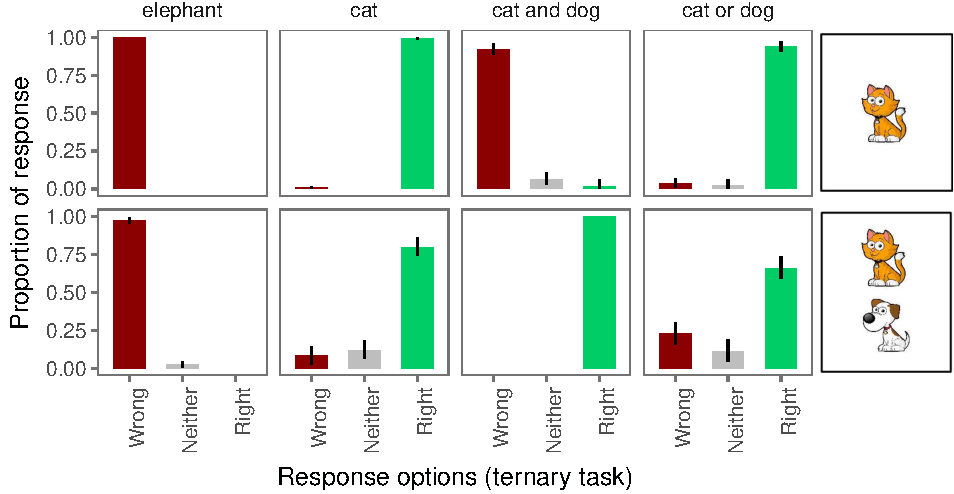
\includegraphics{writeup_files/figure-latex/ternaryPlot-1.pdf}
\caption{\label{fig:ternaryPlot}Proportion responses for the
three-alternative (ternary) forced choice judgments in the guessing
game.}
\end{figure}

Figure \ref{fig:ternaryPlot} shows the proportion of \enquote{right},
\enquote{neither}, and \enquote{wrong} responses in the ternary task.
Similar to the binary task, participants considered a guess wrong when
the mentioned animal was not on the card. They considered the guess
\enquote{right} when the mentioned animal was on the card. However, in
exhaustive trials when the fictional character only guessed one of the
two animals on the card, participants considered the guess
\enquote{wrong} 8\% of the time and neither wrong nor right 12\% of the
time. If a conjunction of animals was guessed and only one animal was
present on the card, participants considered the guess \enquote{wrong}.
As expected, when a conjunction was used and both animals were present,
participants considered the guess \enquote{right}. Similarly,
participants considerd the guess \enquote{right} when a disjunction was
used and only one of the animals was on the card. However, in scalar
trials that both animals were on the card and a disjunction was
gueassed, participants judged the guess \enquote{wrong} 23\% of the time
and \enquote{neither} 11\% of the time.

\begin{figure}
\centering
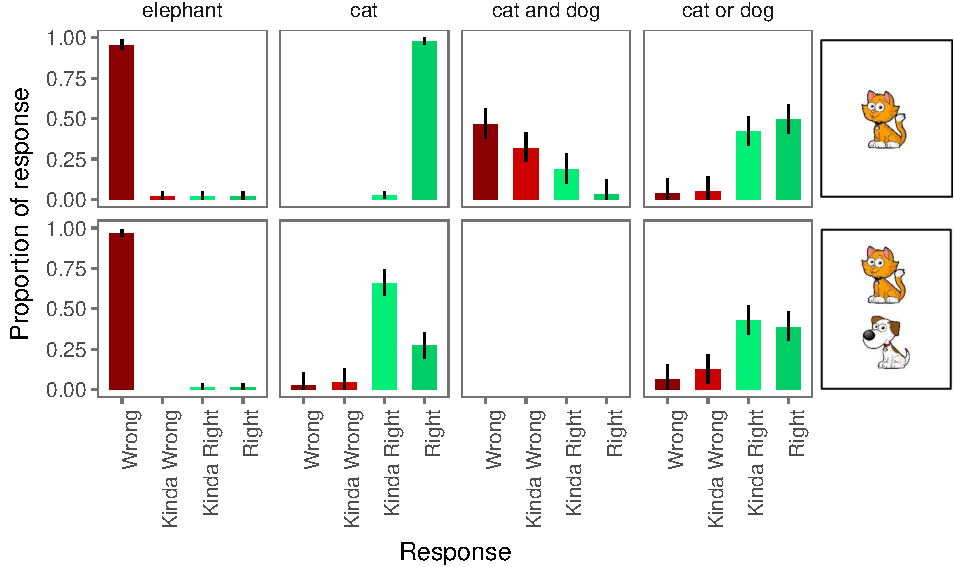
\includegraphics{writeup_files/figure-latex/quaternaryPlot-1.pdf}
\caption{\label{fig:quaternaryPlot}Proportion responses for the
four-alternative (quatenary) forced choice judgments in the guessing
game.}
\end{figure}

Figure \ref{fig:quaternaryPlot} shows the proportion of \enquote{right},
\enquote{kinda right}, \enquote{kinda wrong}, and \enquote{wrong}
responses in the quaternary task. Similar to the results seen
previously, the control trials turned outas expected. Participants
considered a guess \enquote{wrong} if the animal guessed was not on the
card and \enquote{right} if it was the only animal on the card. If a
conjunctin of animals was guessed and both animals were on the card the
guess was \enquote{right}. However, when only one of the animals on the
card was guessed (exhaustive trials), participants judged the guess
\enquote{wrong} 2\% of the time, \enquote{kinda wrong} 5\% of the time,
and \enquote{kinda right} 66\% of the times. Perhaps surprisingly, when
a conjunction was used and only one of the animals was on the card,
participants considered the guess \enquote{wrong} most of the time, but
they often considered it \enquote{kinda wrong} or even \enquote{kinda
right}. This suggests that perhaps participants considered a notion of
partially true or correct statement in our experimental setting.
Disjunctive guesses with one or two animals on the card showed similar
response patterns with participants choosing the \enquote{kinda right}
and \enquote{right} options most of the time. When both animals were on
the card with a disjunctive guess (scalar trials), participants judged
the guess \enquote{wrong} 6\% of the time, \enquote{kinda wrong} 12\% of
the time, and \enquote{kinda right} 43\% of the times.

\begin{figure}
\centering
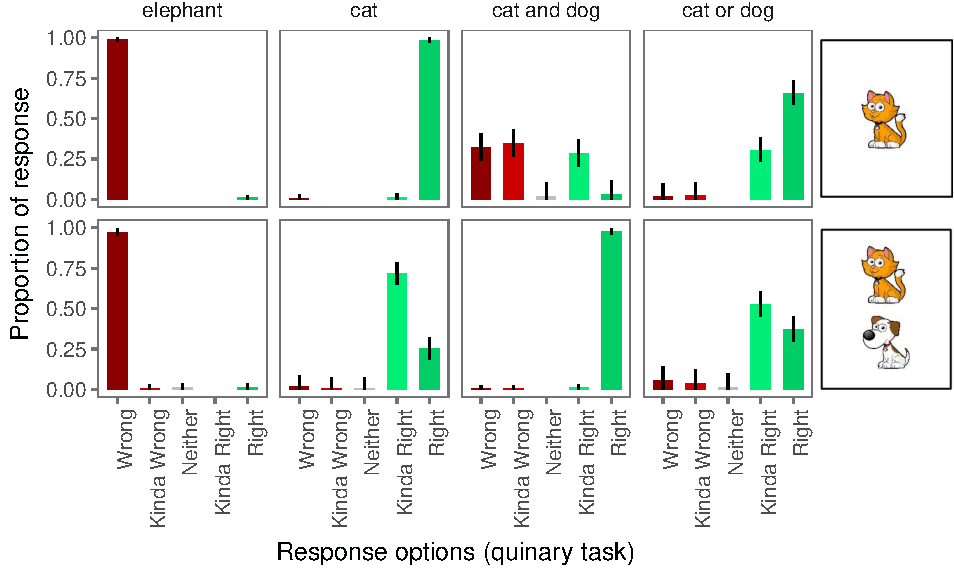
\includegraphics{writeup_files/figure-latex/quinaryPlot-1.pdf}
\caption{\label{fig:quinaryPlot}Proportion responses for the
five-alternative (quinary) forced choice judgments in the guessing
game.}
\end{figure}

Finally, Figure \ref{fig:quinaryPlot} shows the proportion of
\enquote{right}, \enquote{kinda right}, \enquote{neither},
\enquote{kinda wrong}, and \enquote{wrong} responses in the quinary
task. Since the results for the control trials were identical to
previous tasks, we do not repeat them here. In exhaustive trials where
two animals were on the card and only one of them was guessed,
participants chose \enquote{kinda right} the majority of times (72\%).
Again perhaps surprisingly, when only one animal was on the card and the
guess was a conjunction, responses were equally split among
\enquote{wrong}, \enquote{kinda wrong}, and \enquote{kinda right}
responses. With disjunctive guesses, partitipants were more likely to
choose \enquote{right} and \enquote{kinda right} options. When only one
animal was on the card, participants considered the disjunctive guess as
\enquote{right} more often. When both animals were on the card (scalar
trials), participants judged the disjunctive guess as \enquote{kinda
right} 52\% of the time.

Comparing the response patterns in binary to quinary tasks (Figures
\ref{fig:binaryPlot} to \ref{fig:quinaryPlot}), we can observe that in
implicature trials, participants are less likely to choose the endpoints
of the scale (i.e. \enquote{wrong} and \enquote{right}) as they are
given more intermediate options. This raises the possibilty that the
strict \enquote{wrong/right} responses in the tasks with fewer options
(binary and ternary) were not accurately reflecting participant
judgments of implicature trials and pushed their judgments to the
extreme ends. More generally, the data suggest that participant
judgments in contexts that give rise to implicatures fall within the
intermrediate level of the response scale and forced choice tasks with
few options (especially binary tasks) may risk depicting judgments more
extreme than they actually are.

\subsection{Analysis}\label{analysis}

Our primary goal in this study was to check whether the estimated
\enquote{implicature rate} in the experimental task is affected by the
linking assumption and the number of response options available in the
task. Our analysis in this section focuses on these three elements. As
mentioned before, two trial types were predicted to include pragmatic
implicatures. First, trials where two animals were on the card but the
fictional character guessed with a disjunction (scalar); for example
\enquote{cat or dog} when the card has both a cat and a dog on it.
Second, trials where there were two animals on the card but the
character guessed only one (exhaustive); for example \enquote{cat} when
the card had a cat and a dog on it. We called such trials
\enquote{exhaustive}. In our assessment of implicature rate, we focus on
these two trial types.

We considered two linking assumptions. First we defined a weak (lenient)
linking assumption in which any response lower than the maximum point on
the scale (i.e. \enquote{right}) is considered evidence for implicature
computation. Second, we defined a strong (strict) linking assumption
that only considered the lowest point on the scale (i.e.
\enquote{wrong}) as evidence for implicature computation. For each
condition in our study (binary, ternary, quaternary, and quinary) and
each implicature trial type (exhaustive and scalar), we computed a weak
and a strong implicature rate. Figure \ref{fig:implicatureRatePlot}
shows these computed rates.

Comparing the strong and weak rows on Figure
\ref{fig:implicatureRatePlot}, we see that a weak linking assumption
tends to estimate higher implicature rates, especially in tasks with
more response options. With a strong linking assumption, the binary and
possibly ternary judgment tasks derive higher implicature rates than
quaternary and quinary tasks. With a weak linking assumption, the
pattern is reversed. Quaternary and quinary tasks estimate higher rates
than binary and ternary tasks. The patterns show that estimates of
\enquote{implicature rate} depend on linking assumptions and the number
of responses available to participants in the study.

Comparing the exhaustive and scalar columns of Figure
\ref{fig:implicatureRatePlot}, we see that with a strong linking
assumption, there are slightly higher rates for scalar implicatures in
the binary and ternary tasks. With a weak linking assumption, there may
be slightly higher rates for scalar implicatures in the binary and
ternary while the rates may be lower in the quaternary and quinary
tasks. In what follows, we test the effect of linking assumption and
response options on exhaustive and scalar implicature rates more
formally.

\begin{figure}
\centering
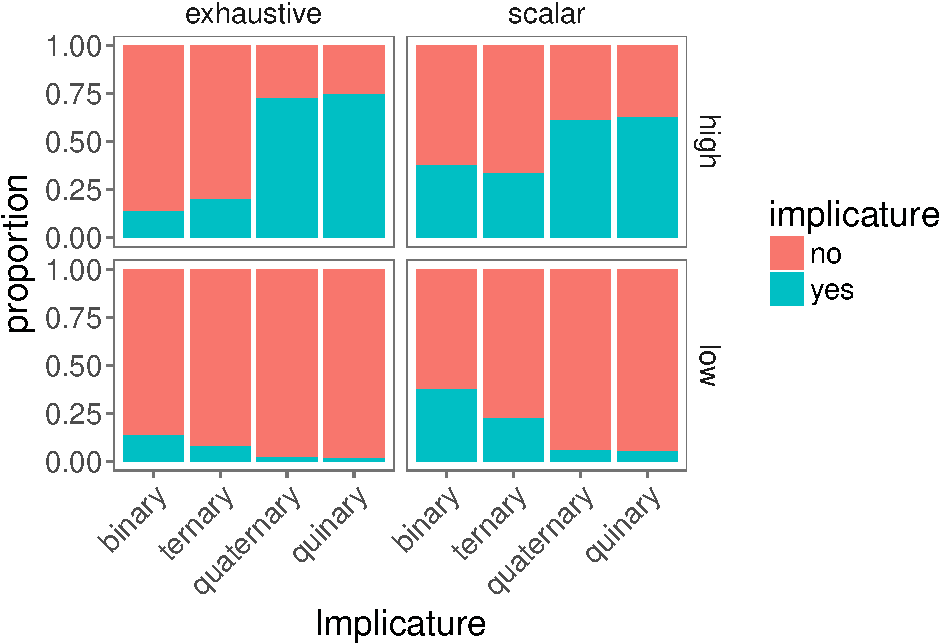
\includegraphics{writeup_files/figure-latex/implicatureRatePlot-1.pdf}
\caption{\label{fig:implicatureRatePlot}Implicature rate in exhaustive and
scalar trials of the binary, ternary, quaternary, and quinary versions
of the guessing game, computed once with a strong linking assumption and
once with a weak linking assumption.}
\end{figure}

For our formal analysis, we use a binomial mixed effects model with the
fixed effect of response type (binary, ternary, quaternary, quinary),
linking assumption (strong vs.~weak), and trial type (exhaustive
vs.~scalar), as wellas the random intercept for participants as well as
random intercept and slope for items (the card they saw).

All the analytical decisions described here were pre-registered and you
can access them through the following link:
\url{https://aspredicted.org/tq3sz.pdf}

\begin{itemize}
\tightlist
\item
  Was logical training a significant predictor of \enquote{implicature
  rate}?
\end{itemize}

\section{\# Discussion}\label{discussion}

On the traditional view of the link between implicature and behavior in
sentence verification tasks, scalar implicature is conceptualized as a
binary, categorical affair - that is, an implicature is either
\enquote{calculated} or it isn't, and the behavioral reflexes of this
categorical interpretation process should be straightforwardly observed
in experimental paradigms. This assumption has concerning implications
for how we must approach analysis of variation in behavior on a truth
value judgment task; for example, why did the majority of respondents in
the binary condition of our experiment answer \enquote{Right} to an
utterance of cat or dog when the card had both a cat and a dog on it?

To explain the data on the traditional view, are forced to say that a)
not all participants calculated the implicature; or that b) some
participants who calculated the implicature did not choose the
anticipated response (i.e. \enquote{Wrong}) due to some other cognitive
reflex which \enquote{overrode} the implicature; or some mixture of (b)
and (c). We might similarly posit that one or both of these factors
underlie the variation in the ternary, quatenary, and quinary conditions
(e.g.~why were participants roughly split between \enquote{Right} and
\enquote{Kind of right} when the utterance was cat or dog and the card
had a cat and a dog?). However, the best we can hope for on this
approach is an analysis which traces the general qualitative patterns in
the data.

We contrast the above view of implicature and its behavioral reflexes
with an alternative linking hypothesis which assumes that participants'
behavior can be represented using the model of a soft-optimal pragmatic
speaker in the RSA framework. This alternative linking hypothesis
contrasts with the traditional view in it is rooted in a quantitative
formalization of pragmatic competence which provides us a continuous
measure of pragmatic reasoning. Recall that in RSA, pragmatically
competent listeners are modeled as a continuous probabilistic
distribution of possible meanings given an utterance which that listener
hears. The probability with which this listener \(L_1\) ascribes a
meaning s to an utterance u depends upon a prior probability
distribution of potential states of the world \(P_w\), and upon
reasoning about the communicative behavior of a speaker \(S_1\). \(S_1\)
in turn is modeled as a continuous probabilistic distribution of
possible utterances given an intended state of affairs the speaker
intends to communicate. This distribution is sensitive to a rationality
parameter \(\alpha\), the production cost \(C\) of potential utterances,
and a representation of a literal listener \(L_0\) whose interpretation
of an utterance is in turn a function of that utterance's truth
conditional content \([[u]](s)\) and her prior beliefs about the state
of the world \(P_w(s)\).

\begin{verbatim}
$P_{L_1}(s | u) \propto P_{S_1}(u | s) * P_w(s)$

$P_{S_1}(u | s) \propto exp(\alpha(log(L_0(s | u)) - C(u))) $

$P_{L_0}(s | u) \propto [[u]](s) * P_w(s)$
\end{verbatim}

In this framework, individuals never categorically draw (or fail to
draw) pragmatic inferences about the utterances they hear. For example,
exclusivity readings of disjunction or are represented in RSA as
relatively low conditional probability of a conjunctive meaning on the
\(P_L\) distribution, given an utterance of or. Thus, it is not even
possible to talk about \enquote{rate} of implicature calculation in the
RSA framework. The upshot, as we show below, is that this view of
pragmatic competence does allow us to talk explicitly and quantitatively
about rates of observed behavior in sentence verification tasks.

First, following Degen \& Goodman (2014), we proceed on the assumption
that behavior on sentence verification tasks, such as truth value
judgment tasks, is best modeled as a function of an individual's mental
representation of a cooperative interlocutor (\(S_1\) in the language of
RSA) rather than of a pragmatic listener who interprets utterances
(\(P_{L_1}\)). In their paper, Degen \& Goodman argue that sentence
verification tasks are relatively more sensitive to contextual
manipulations (such as manipulation of the Question Under Discussion)
than are sentence interpretation tasks, and that this follows if
sentence interpretation tasks - but not sentence verification tasks -
require an additional layer of counterfactual reasoning about the
intentions of a cooperative speaker.

A main desideratum of a behavioral linking hypothesis given the RSA view
of pragmatic competence is to transform continuous probability
distributions into categorical outputs (e.g.~responses of
\enquote{Right}/''Wrong'' in the case of the binary condition of our
experiment). For a given utterance u and an intended communicated
meaning w, \(S_1\)(u \textbar{} w) outputs a conditional probability of
u given w. For example, in the binary condition of our experiment where
a participant evaluated cat or dog when there were both animals on the
card, the participant has access to the mental representation of \(S_1\)
and hence to the \(S_1\) conditional probability of hearing the
utterance cat or dog given a dog and cat card: \(S_1\)(cat or dog
\textbar{} cat and dog). According to the linking hypothesis advanced
here, the participant provides a particular response to u if the RSA
speaker probability of u lies within a particular probability interval,
given an observed state of the world (i.e.~the configuration of animals
on the card in our experiment). We model a responder, R, who in the
binary condition responds \enquote{Right} to an utterance u in world w
just in case \(S_1\)(u \textbar{} w) exceeds some probability threshold
\(\theta\):

R(u, w, \(\theta\))

= \enquote{Right} iff \(S_1\)(u \textbar{} w) \(>\) \(\theta\)

= \enquote{Wrong} otherwise

In the experiment conditions where there are more than two choices, we
model the range of possible behavioral responses for R with the
introduction of intermediate probability thresholds. For example, in the
ternary condition, R(u, w, \(\theta_1\) , \(\theta_2\)) is
\enquote{Right} iff \(S_1\)(u \textbar{} w) \textgreater{} \(\theta_1\)
and \enquote{Neither} iff \(\theta_1\) \textgreater{} \(S_1\)(u
\textbar{} w) \textgreater{} \(\theta_2\). To fully generalize the model
to our five experimental conditions, we say that R takes as its input an
utterance u, a world state w, and a number of threshold variables
dependent on a variable c, corresponding to the experimental condition
in which the participant finds herself (e.g.~the range of possible
responses available to R).

Given c = \enquote{ternary}

R(u, w, \(\theta_1\) , \(\theta_2\))

= \enquote{Right} iff \(S_1\)(u \textbar{} w) \(>\) \(\theta_1\)

= \enquote{Neither} iff \(\theta_1\) \(>\) \(S_1\)(u \textbar{} w) \(>\)
\(\theta_2\)

= \enquote{Wrong} otherwise

Given c = \enquote{quatenary}

R(u, w, \(\theta_1\) , \(\theta_2\), \(\theta_3\))

= \enquote{Right} iff \(S_1\)(u \textbar{} w) \(>\) \(\theta_1\)

= \enquote{Kinda Right} iff \(\theta_1\) \(>\) \(S_1\)(u \textbar{} w)
\(>\) \(\theta_2\)

= \enquote{Kinda Wrong} iff \(\theta_2\) \(>\) \(S_1\)(u \textbar{} w)
\(>\) \(\theta_3\)

= \enquote{Wrong} otherwise

Given c = \enquote{quinary}

R(u, w, \(\theta_1\) , \(\theta_2\), \(\theta_3\). \(\theta_4\))

= \enquote{Right} iff \(S_1\)(u \textbar{} w) \(>\) \(\theta_1\)

=\enquote{Kinda Right} iff \(\theta_1\) \(>\) \(S_1\)(u \textbar{} w)
\(>\) \(\theta_2\)

= \enquote{Neither} iff \(\theta_2\) \(>\) \(S_1\)(u \textbar{} w) \(>\)
\(\theta_3\)

= \enquote{Kinda Wrong} iff \(\theta_3\) \(>\) \(S_1\)(u \textbar{} w)
\(>\) \(\theta_4\)

= \enquote{Wrong} otherwise

Bayesian statistical methods provide us a means for estimating the
values of these probability thresholds in our RSA model. The basis for
the model is a set of possible states of the world, given a universe of
three animals - X, Y, and Z - that each may be on some card. We next
define a set of possible sentences a speaker might utter, assuming the
speaker intends to communicate which animals are on the card. We assume
a uniform prior probability of different states of the world and a
uniform cost function on utterances. We define a literal listener
\(L_0\), a pragmatic speaker \(S_1\), and a responder \(R\) according to
our definitions above. Lastly, and assuming a uniform prior distribution
over possible values of probability thresholds, we use Bayesian
inference to recover a posterior distribution of these thresholds in
each experimental condition, given the actual observed rate of response
in each condition of the experiment. The results of this parameter
estimation analysis are shown in the figures below, where the X axis of
each figure corresponds to a threshold value between 0 and 1 and the Y
axis corresponds to the posterior probability density of possible values
of the threshold.

\begin{verbatim}
## Warning in is.na(e1) | is.na(e2): longer object length is not a multiple of
## shorter object length
\end{verbatim}

\begin{verbatim}
## Warning in `==.default`(Parameter, c("quatenary_theta1",
## "quatenary_theta2", : longer object length is not a multiple of shorter
## object length
\end{verbatim}

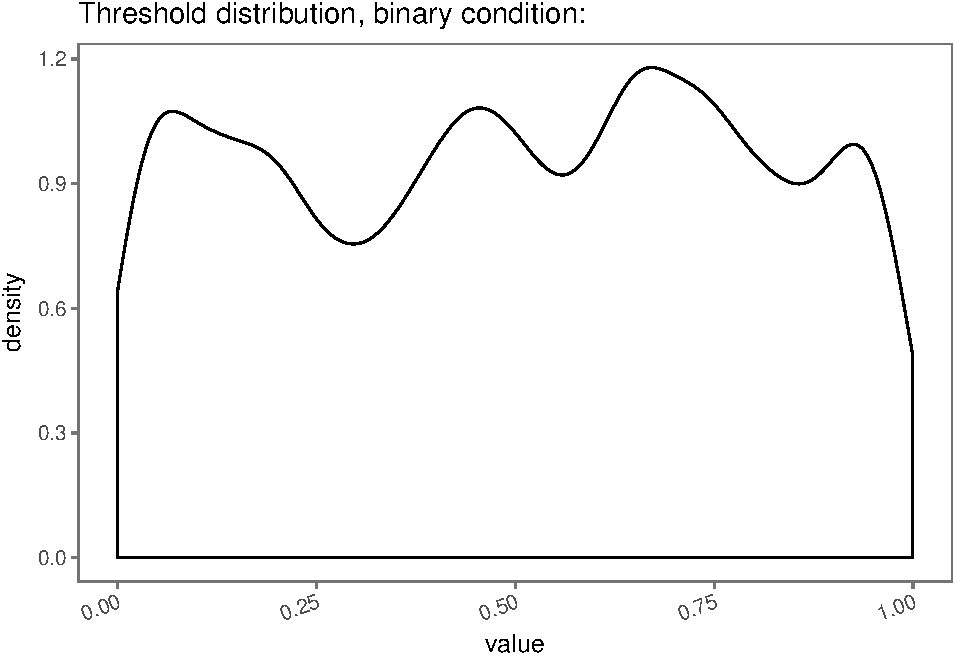
\includegraphics{writeup_files/figure-latex/unnamed-chunk-1-1.pdf}
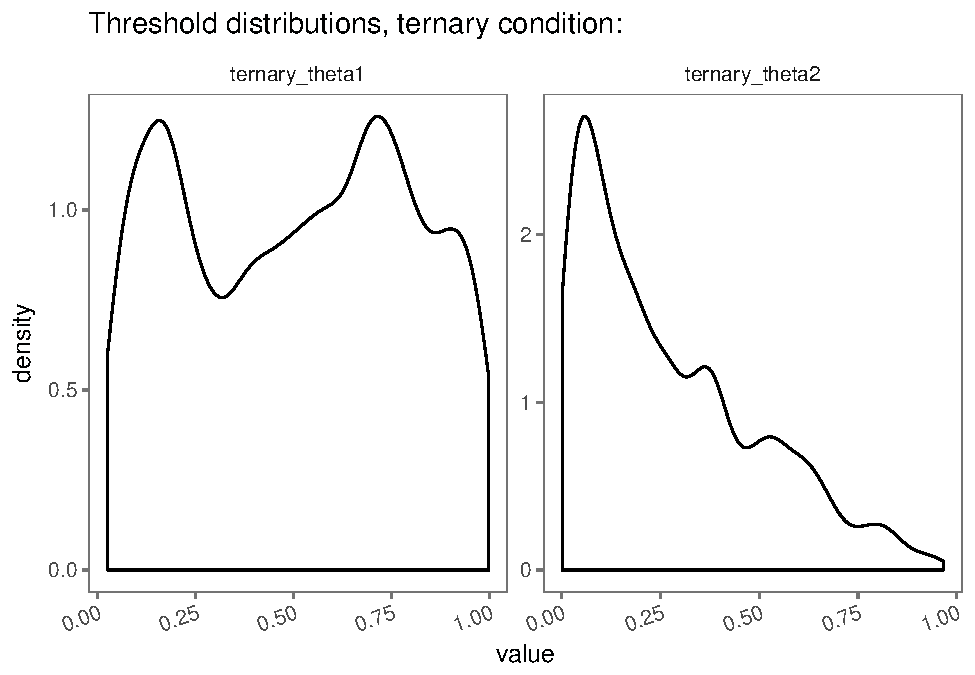
\includegraphics{writeup_files/figure-latex/unnamed-chunk-1-2.pdf}
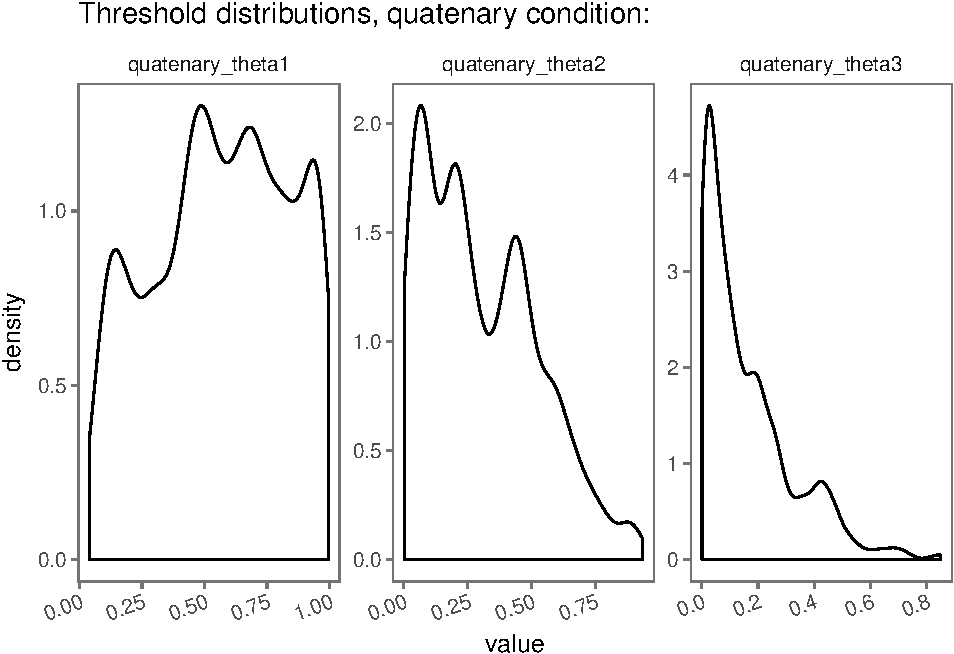
\includegraphics{writeup_files/figure-latex/unnamed-chunk-1-3.pdf}
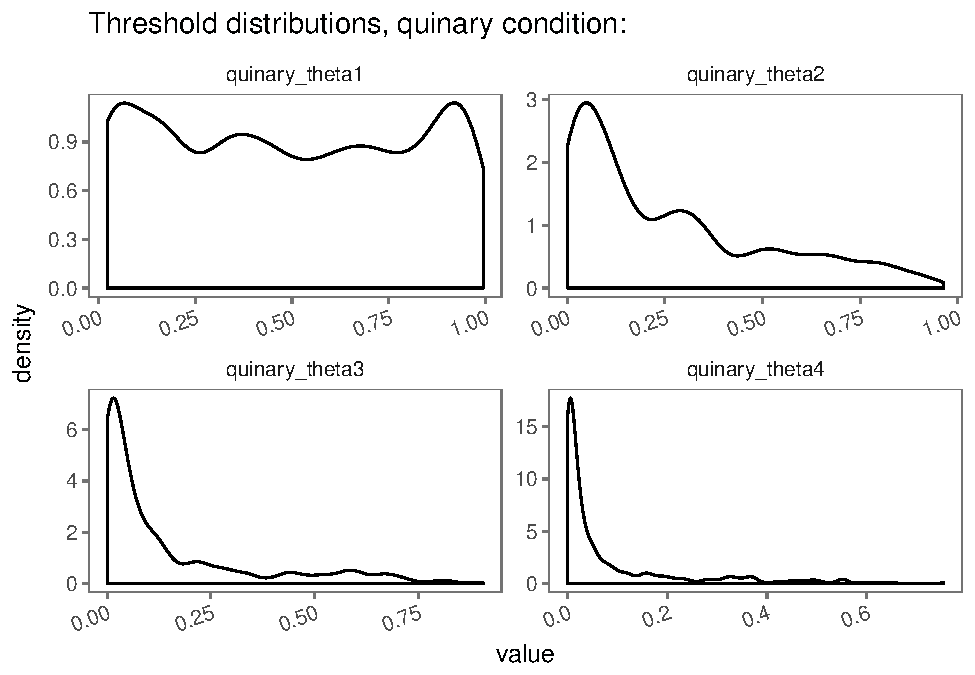
\includegraphics{writeup_files/figure-latex/unnamed-chunk-1-4.pdf}

The above analysis is a proof of concept for the following idea: by
relaxing the assumptions of the traditional view of scalar implicature
(namely, that scalar implicatures either are or are not calculated, and
that behavior on sentence verification tasks directly reflects this
binary interpretation process), we can propose quantitative models of
the variation in behavior we observe in experimental settings.

\section{References}\label{references}

\setlength{\parindent}{-0.5in} \setlength{\leftskip}{0.5in}

\hypertarget{refs}{}
\hypertarget{ref-Barner2011}{}
Barner, D., Brooks, N., \& Bale, A. (2011). Accessing the unsaid: the
role of scalar alternatives in children's pragmatic inference.
\emph{Cognition}, \emph{118}(1), 84--93.
doi:\href{https://doi.org/10.1016/j.cognition.2010.10.010}{10.1016/j.cognition.2010.10.010}

\hypertarget{ref-Bergen2012}{}
Bergen, L., \& Grodner, D. J. (2012). Speaker knowledge influences the
comprehension of pragmatic inferences. \emph{Journal of Experimental
Psychology. Learning, Memory, and Cognition}, \emph{38}(5), 1450--60.
doi:\href{https://doi.org/10.1037/a0027850}{10.1037/a0027850}

\hypertarget{ref-Bonnefon2009}{}
Bonnefon, J.-F., Feeney, A., \& Villejoubert, G. (2009). When some is
actually all: scalar inferences in face-threatening contexts.
\emph{Cognition}, \emph{112}(2), 249--58.
doi:\href{https://doi.org/10.1016/j.cognition.2009.05.005}{10.1016/j.cognition.2009.05.005}

\hypertarget{ref-Bott2004}{}
Bott, L., \& Noveck, I. (2004). Some utterances are underinformative:
The onset and time course of scalar inferences. \emph{Journal of Memory
and Language}, \emph{51}(3), 437--457.
doi:\href{https://doi.org/10.1016/j.jml.2004.05.006}{10.1016/j.jml.2004.05.006}

\hypertarget{ref-Breheny2013}{}
Breheny, R., Ferguson, H. J., \& Katsos, N. (2013). Taking the epistemic
step: Toward a model of on-line access to conversational implicatures.
\emph{Cognition}, \emph{126}(3), 423--40.
doi:\href{https://doi.org/10.1016/j.cognition.2012.11.012}{10.1016/j.cognition.2012.11.012}

\hypertarget{ref-Breheny2006}{}
Breheny, R., Katsos, N., \& Williams, J. (2006). Are generalised scalar
implicatures generated by default? An on-line investigation into the
role of context in generating pragmatic inferences. \emph{Cognition},
\emph{100}(3), 434--63.
doi:\href{https://doi.org/10.1016/j.cognition.2005.07.003}{10.1016/j.cognition.2005.07.003}

\hypertarget{ref-Chemla2011}{}
Chemla, E., \& Spector, B. (2011). Experimental Evidence for Embedded
Scalar Implicatures. \emph{Journal of Semantics}, \emph{28}(3),
359--400.

\hypertarget{ref-DeNeys2007}{}
De Neys, W., \& Schaeken, W. (2007). When People Are More Logical Under
Cognitive Load - Dual Task Impact on Scalar Implicature.
\emph{Experimental Psychology}, \emph{54}(2), 128--133.
doi:\href{https://doi.org/10.1027/1618-3169.54.2.128}{10.1027/1618-3169.54.2.128}

\hypertarget{ref-Degen2015}{}
Degen, J. (2015). Investigating the distribution of 'some' (but not
'all') implicatures using corpora and web-based methods. \emph{Semantics
and Pragmatics}, \emph{8}(11), 1--55.
doi:\href{https://doi.org/10.3765/sp.8.11}{10.3765/sp.8.11}

\hypertarget{ref-Degen2014}{}
Degen, J., \& Goodman, N. D. (2014). Lost your marbles? The puzzle of
dependent measures in experimental pragmatics. \emph{Proceedings of the
36th Annual Conference of the Cognitive Science Society}, 397--402.

\hypertarget{ref-DegenTanenhaus2015}{}
Degen, J., \& Tanenhaus, M. K. (2015). Processing scalar implicature A
constraint-based approach. \emph{Cognitive Science}, \emph{39}(4),
667--710.
doi:\href{https://doi.org/10.1111/cogs.12171}{10.1111/cogs.12171}

\hypertarget{ref-DegenTanenhaus2016}{}
Degen, J., \& Tanenhaus, M. K. (2016). Availability of Alternatives and
the Processing of Scalar Implicatures: A Visual World Eye-Tracking
Study. \emph{Cognitive Science}, \emph{40}(1), 172--201.
doi:\href{https://doi.org/10.1111/cogs.12227}{10.1111/cogs.12227}

\hypertarget{ref-Doran2012}{}
Doran, R., Ward, G., Larson, M., McNabb, Y., \& Baker, R. E. (2012). A
novel experimental paradigm for distinguishing between what is said and
what is implicated. \emph{Language}, \emph{88}, 124--154.

\hypertarget{ref-Geurts2009}{}
Geurts, B., \& Pouscoulous, N. (2009). Embedded implicatures?!?
\emph{Semantics and Pragmatics}, \emph{2}, 1--34.
doi:\href{https://doi.org/10.3765/sp.2.4}{10.3765/sp.2.4}

\hypertarget{ref-grice1975}{}
Grice, H. P. (1975). Logic and Conversation. \emph{Syntax and
Semantics}, \emph{3}, 41--58. Retrieved from
\href{http://books.google.com/books?hl=en\%7B/\&\%7Dlr=\%7B/\&\%7Did=hQCzOmaGeVYC\%7B/\&\%7Doi=fnd\%7B/\&\%7Dpg=PA121\%7B/\&\%7Ddq=Logic+and+conversation\%7B/\&\%7Dots=j7aijUymwm\%7B/\&\%7Dsig=iV1rz1eEm4ns6bQ6CevIURXFVO4}{http://books.google.com/books?hl=en\{\textbackslash{}\&\}lr=\{\textbackslash{}\&\}id=hQCzOmaGeVYC\{\textbackslash{}\&\}oi=fnd\{\textbackslash{}\&\}pg=PA121\{\textbackslash{}\&\}dq=Logic+and+conversation\{\textbackslash{}\&\}ots=j7aijUymwm\{\textbackslash{}\&\}sig=iV1rz1eEm4ns6bQ6CevIURXFVO4}

\hypertarget{ref-Grodner2010}{}
Grodner, D. J., Klein, N. M., Carbary, K. M., \& Tanenhaus, M. K.
(2010). ``Some,'' and possibly all, scalar inferences are not delayed:
Evidence for immediate pragmatic enrichment. \emph{Cognition},
\emph{116}(1), 42--55.
doi:\href{https://doi.org/10.1016/j.cognition.2010.03.014}{10.1016/j.cognition.2010.03.014}

\hypertarget{ref-horn1984}{}
Horn, L. (1984). Toward a new taxonomy for pragmatic inference: Q-based
and R-based implicature. In D. Schiffrin (Ed.), \emph{Meaning, form, and
use in context: Linguistic applications} (pp. 11--42). Washington:
Georgetown University Press.

\hypertarget{ref-huang2009}{}
Huang, Y. T., \& Snedeker, J. (2009). On-line interpretationf of scalar
quantifiers: Insight into the semantics-pragmatics interface.
\emph{Cognitive Psychology}, \emph{58}, 376--415.

\hypertarget{ref-Katsos2011}{}
Katsos, N., \& Bishop, D. V. M. (2011). Pragmatic tolerance:
implications for the acquisition of informativeness and implicature.
\emph{Cognition}, \emph{120}(1), 67--81.
doi:\href{https://doi.org/10.1016/j.cognition.2011.02.015}{10.1016/j.cognition.2011.02.015}

\hypertarget{ref-levinson2000}{}
Levinson, S. C. (2000). \emph{Presumptive Meanings - The Theory of
Generalized Conversational Implicature}. MIT Press.

\hypertarget{ref-DeMarneffe2017}{}
Marneffe, M.-C. de, \& Tonhauser, J. (2016). Inferring meaning from
indirect answers to polar questions: The contribution of the
rise-fall-rise contour. In E. Onea, M. Zimmermann, \& K. von Heusinger
(Eds.), \emph{Questions in discourse}. Leiden: Brill Publishing.

\hypertarget{ref-Musolino2004}{}
Musolino, J. (2004). The semantics and acquisition of number words:
integrating linguistic and developmental perspectives. \emph{Cognition},
\emph{93}(1), 1--41.
doi:\href{https://doi.org/10.1016/j.cognition.2003.10.002}{10.1016/j.cognition.2003.10.002}

\hypertarget{ref-Noveck2001}{}
Noveck, I. (2001). When children are more logical than adults:
experimental investigations of scalar implicature. \emph{Cognition},
\emph{78}(2), 165--188. Retrieved from
\url{http://www.ncbi.nlm.nih.gov/pubmed/11074249}

\hypertarget{ref-noveck2008}{}
Noveck, I. A., \& Reboul, A. (2008). Experimental pragmatics: a Gricean
turn in the study of language. \emph{Trends in Cognitive Sciences},
\emph{12}(11), 425--431.
doi:\href{https://doi.org/10.1016/j.tics.2008.07.009}{10.1016/j.tics.2008.07.009}

\hypertarget{ref-Noveck2003}{}
Noveck, I., \& Posada, A. (2003). Characterizing the Time Course of an
Implicature: an Evoked Potentials Study. \emph{Brain and Language},
\emph{85}(2), 203--210.
doi:\href{https://doi.org/10.1016/S0093-934X(03)00053-1}{10.1016/S0093-934X(03)00053-1}

\hypertarget{ref-Papafragou2004}{}
Papafragou, A., \& Tantalou, N. (2004). Children's Computation of
Implicatures. \emph{Language Acquisition}, \emph{12}(1), 71--82.

\hypertarget{ref-Politzer-Ahles2013}{}
Politzer-Ahles, S., \& Fiorentino, R. (2013). The Realization of Scalar
Inferences: Context Sensitivity without Processing Cost. \emph{PLoS
ONE}, \emph{8}(5).
doi:\href{https://doi.org/10.1371/journal.pone.0063943}{10.1371/journal.pone.0063943}

\hypertarget{ref-VanTiel2014}{}
Tiel, B. van, Miltenburg, E. van, Zevakhina, N., \& Geurts, B. (2014).
Scalar diversity. \emph{Journal of Semantics}.
doi:\href{https://doi.org/10.1093/jos/ffu017}{10.1093/jos/ffu017}

\hypertarget{ref-Zondervan2010}{}
Zondervan, A. (2010). \emph{Scalar implicatures or focus: an
experimental approach} (PhD thesis). Universiteit Utrecht, Amsterdam.






\end{document}
